\documentclass[conference]{IEEEtran}

\usepackage[T1]{fontenc}
\usepackage{amsmath,amssymb}
\usepackage{booktabs}
\usepackage{array}
\usepackage{enumitem}
\usepackage{cite}
\usepackage{tikz}
\usetikzlibrary{arrows.meta,positioning,fit,backgrounds,calc,patterns}
\usepackage[hidelinks]{hyperref}
\newcommand{\doi}[1]{doi:\,\url{#1}}

\setlist{itemsep=1pt,topsep=2pt,leftmargin=*}
\newcommand{\todo}[1]{\textcolor{red!70!black}{[#1]}}
\usepackage{xcolor}

\begin{document}

\title{Change-Characteristic-Aware Window Selection for Unsupervised Concept Drift Detection in Real-Time Text Streams}

\makeatletter
\newcommand{\linebreakand}{\end{@IEEEauthorhalign}\hfill\mbox{}\par\mbox{}\hfill\begin{@IEEEauthorhalign}}
\makeatother

% \author{
% \IEEEauthorblockN{Md. Abu Towsif}
% \IEEEauthorblockA{26-93964-1@student.aiub.edu\\
% American International\\University-Bangladesh}
% \and
% \IEEEauthorblockN{Farjana Yesmin Opi}
% \IEEEauthorblockA{{26-93965-1@student.aiub.edu}\\
% American International\\University-Bangladesh}
% \and
% \IEEEauthorblockN{Mst. Nadiya Noor}
% \IEEEauthorblockA{{26-94277-3@student.aiub.edu}\\
% American International\\University-Bangladesh}
% \linebreakand
% \IEEEauthorblockN{Md. Jahid Hasan}
% \IEEEauthorblockA{{26-94240-@student.aiub.edu}\\
% American International\\University-Bangladesh}
% \and
% \IEEEauthorblockN{Hasibur Rashid Chayon}
% \IEEEauthorblockA{{chayon@aiub.edu}\\
% American International\\University-Bangladesh}
% }

\maketitle

%--------------------------------------------------------------------
\section{Introduction}

Text is produced continuously by news feeds, review sites and social platforms. Their topics and vocabulary change over time and a model trained on older documents slowly becomes outdated. For example a news classifier encounters new subjects and terms after a major event. This change in the data-generating process is called concept drift \cite{gama2014,lu2019}. Real-time systems must notice it because the usual remedy is to update the model on recent data which costs computation and often new annotations. Text streams also show three characteristics of big data. They have high velocity as documents arrive continuously and must be processed in a single pass. They have variety because the documents are unstructured and differ in topic, source and style. And their veracity is uncertain since labels are missing and the true drift points are usually unknown.


For text, the problem is harder because labels arrive late or never \cite{garcia2024review}. Classic detectors watch a classifier's error rate and need the true label after every prediction \cite{gama2004,bifet2007} so a text detector has to work without labels. It should identify a genuine change quickly while avoiding alarms caused by ordinary fluctuations. A late alarm keeps an outdated model in use whereas a false alarm can trigger an unnecessary update and may need additional labeling costs. Lukats et al.\ \cite{lukats2025} showed that accuracy-based scores can favor detectors that fire often, highlighting the need to evaluate detection delay and false alarms separately.

Unsupervised detectors usually compare a window of recent data with a window of older data \cite{hinder2024a}. A short window reacts fast but is sensitive to noise while a long window is stable but slow. The best size also depends on the drift since a gradual or subtle change needs more data to stand out than an abrupt one. The benchmark in \cite{lukats2025} names better window-size selection as open future work.
ADWIN \cite{bifet2007} avoids a fixed size by keeping a variable-length window and cutting it when two parts differ according to a Hoeffding-type bound. It is mostly applied to classifier errors which needs labels. ADWIN-U \cite{assis2025} removes this need by monitoring simple statistics of each example such as skewness and kurtosis which worked best in its tests on ten numeric streams. It is our starting point. Three issues still need to be addressed. These include its fixed confidence level δ, dropping the whole older sub-window after each detection whatever the strength or persistence of the change and evaluation only on numeric sensor-type streams. For text it is not clear whether these statistics can detect topic changes in sentence embeddings.

We study a window-selection policy built on ADWIN-U. At first, the detector looks at how strong and how persistent the unlabeled evidence is and then chooses between a full cut, a hold and a partial cut of the window. It reuses ADWIN's bucketed window so its cost per instance should stay close to that of ADWIN-U. In terms of these characteristics, the policy handles velocity with a compact window that is updated in constant time, variety by working on sentence embeddings of unstructured text and veracity by using no labels and by not acting on a single weak signal. Our work check whether this improves the balance between delay, false alarms and missed drift on text streams and how the effect depends on drift type and magnitude. We also measure how much time and memory it uses and check whether the results from added drift also apply to a real stream where the drift points are unknown.

The main contributions of our work are:
(i) We propose a label-free window-selection policy with a hold state and a graded cut that contains ADWIN-U as a special case at the same $O(\log W)$ cost.
(ii) We show that graded cutting lowers detection delay on gradual and subtle drift at a matched false-alarm rate, while abrupt drift is handled as in ADWIN-U.
(iii) We examine whether ADWIN-U's per-instance statistics capture topic drift in sentence embeddings, compared with a centroid-distance signal.


Our contribution is not the adaptive window or the label-free monitoring itself which ADWIN and ADWIN-U already provide. It is the rule that decides how the window changes after evidence of drift and its evaluation on text.

The rest of the paper is organized as follows. Section~\ref{sec:related} covers related work and Section~\ref{sec:method} explains the proposed method and how we plan to evaluate it.

%--------------------------------------------------------------------
\section{Background and Related Work}
\label{sec:related}

\subsection{Concept drift and its types}

A data stream is a sequence of instances arriving over time. Concept drift occurs between times $t$ and $t+\Delta$ if the joint distribution changes, $P_t(X,Y)\neq P_{t+\Delta}(X,Y)$ \cite{gama2014}. Changes in $P(X)$ alone are called virtual drift or feature change. Detectors that use no labels can only observe this kind \cite{assis2025}. Drift is commonly grouped by its speed and shape into abrupt, gradual, incremental and recurring drift \cite{webb2016,suarez2023}. Abrupt drift replaces one concept by another at a single point. Gradual drift mixes the old and new concept for a period. Recurring drift occurs when a previously seen concept returns such as with seasonal changes. Reviews of the field \cite{gama2014,lu2019} also cover how models are adapted after a detection.

\subsection{Supervised and unsupervised detectors}

Supervised detectors such as DDM \cite{gama2004} and ADWIN \cite{bifet2007} watch the error of a classifier and need the true label soon after each prediction. Assis and Souza note that this is unrealistic in many applications and that unsupervised methods are still a small part of the literature \cite{assis2025}.

Unsupervised detectors compare the distribution of recent and older data. Hinder et al. describe this as a common approach where two windows are selected and each is summarized before testing a dissimilarity score \cite{hinder2024a}. They also list how the reference window can be kept and most approaches use sliding windows. For example, KSWIN which applies the Kolmogorov--Smirnov test inside a sliding window \cite{raab2020} and D3 which trains a classifier to separate old from new instances and watches its AUC \cite{gozuacik2019}. Lukats et al.\ \cite{lukats2025} surveyed ten fully unsupervised detectors and compared seven on eleven real-world streams. No detector won on every metric and classifier accuracy can favor detectors that fire often since frequent updates keep the model fresh. For this reason we report delay and false alarms directly and we use accuracy-based scores only as secondary evidence. The same study suggests automatic selection of window sizes as future work.

\subsection{Adaptive windows}

ADWIN \cite{bifet2007} maintains a window $W$ and examines every split $W=W_1\cdot W_2$. A change is declared when $|\hat\mu_{W_1}-\hat\mu_{W_2}|\ge\varepsilon_{\mathrm{cut}}$ where the bound $\varepsilon_{\mathrm{cut}}$ comes from Hoeffding's inequality \cite{hoeffding1963} and depends on a confidence level $\delta$. Once a change is detected, the older part $W_1$ is dropped. To stay cheap, ADWIN stores the window as an exponential histogram \cite{datar2002} which requires $O(\log W)$ memory and time.

Several other methods follow different strategies for adjusting the window. DAWIDD, for instance, examines the statistical dependence between the observed data and time to determine whether a change has occurred \cite{hinder2020}. Chen et al.\ use a short and a long variable window with a decay model to separate drift types in frequent pattern mining \cite{chen2024}. Klinkenberg and Joachims \cite{klinkenberg2000} and Kuncheva and \v{Z}liobait\.{e} \cite{kuncheva2009} choose the window size from estimated classification error or from theory so they need labels or a classifier. Window handling also appears in applied systems. Mehmood et al.\ combine an LSTM with the Page--Hinkley test, ADWIN and KSWIN for sensor forecasting on an edge architecture \cite{mehmood2024}. Badar et al.\ use EDDM to update a sliding window in federated stream classification \cite{badar2023}. Hu et al.\ adjust a model's enclosing ball by expanding and contracting it so that it follows new concepts without growing too large \cite{hu2024}. These works adjust windows or models in several ways but none of the studies we reviewed defines a general label-free policy for deciding how much of a window to drop.

\subsection{ADWIN-U}

ADWIN-U \cite{assis2025} keeps the ADWIN windowing and replaces the monitored value. From each example it extracts a descriptive statistic $s_i$ (for example skewness or kurtosis over the feature values) and feeds it to ADWIN. It has a single-detector form with one window and a multiple-detector form with one window per predicted class where an alarm in any window restarts all of them. In the authors' tests on ten real numeric streams, skewness and kurtosis worked best with multiple detectors and the geometric mean worked best with a single detector. The cost stays at $O(\log W)$ per instance for one detector and $O(l\log W)$ for $l$ detectors. The authors also propose the BAR score which combines accuracy with the share of labels requested for model updates. They set $\delta=0.002$ in their experiments and suggest monitoring several statistics at once through voting or dynamic selection as future work.

\subsection{Text streams}

Garcia et al.\ reviewed drift adaptation in text stream mining and point out that few text benchmarks come with labeled drift points \cite{garcia2024review}. Text is turned into vectors with pre-trained encoders such as Sentence-BERT \cite{reimers2019}. Whether the simple statistics that work for numeric sensor data also react to topic drift in embeddings has not been tested. To our knowledge, ADWIN-U-style windowing has not been evaluated on text streams although a systematic literature search is still needed to confirm this.

In summary, window choice shapes what a detector sees, ADWIN-U provides a label-free adaptive window and text streams lack a tested evaluation protocol. What is still missing is a rule that uses the strength and persistence of unlabeled evidence to decide how the window changes and an evaluation of that rule on text.

%--------------------------------------------------------------------
\section{Proposed Methodology}
\label{sec:method}

\begin{figure*}[!t]
\centering
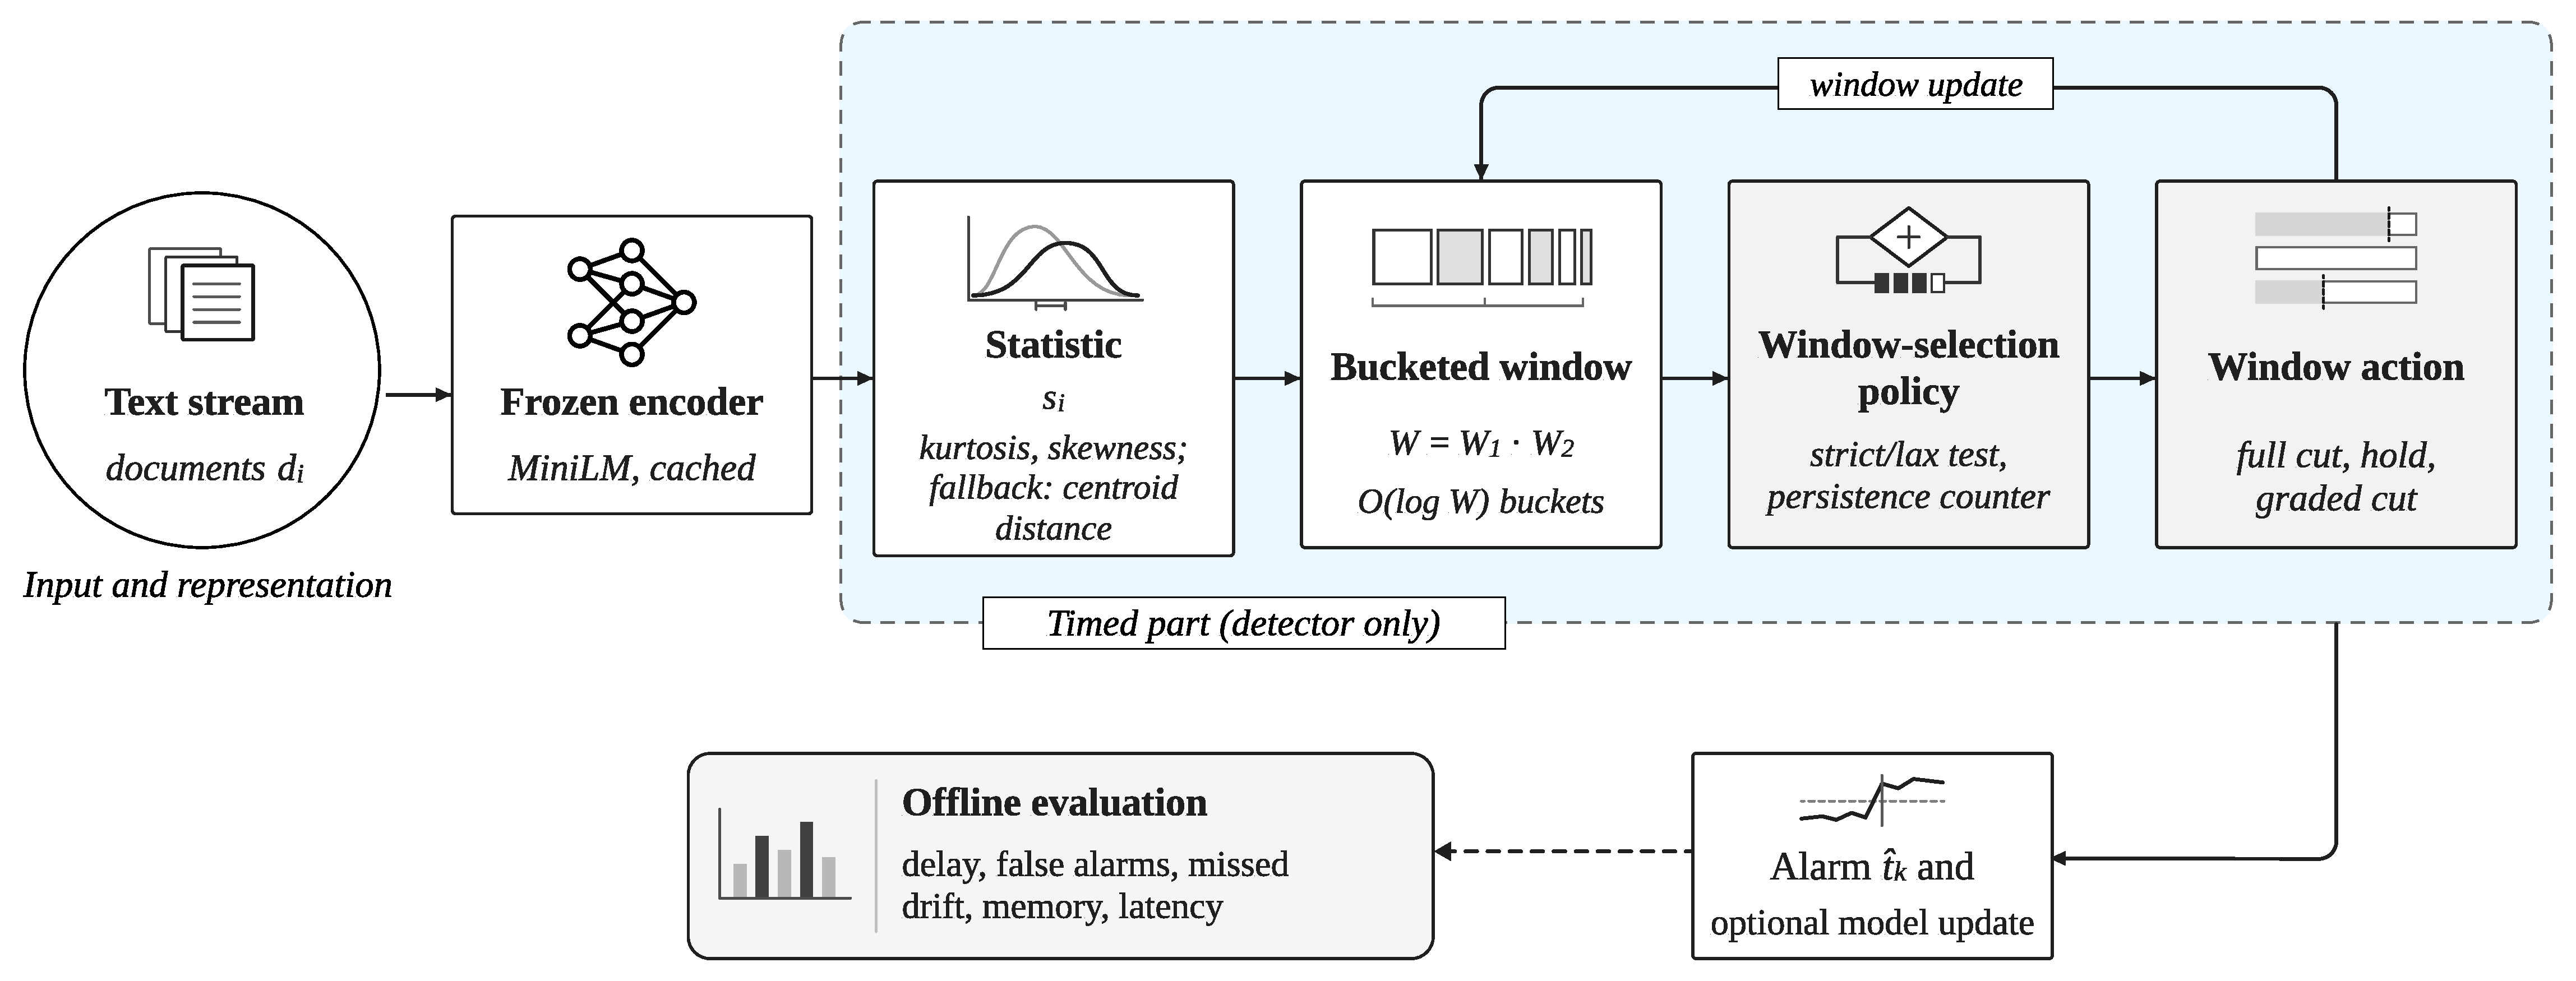
\includegraphics[width=\linewidth]{figures/pipeline.pdf}
\caption{Overview of the proposed pipeline. Embeddings are computed once and cached ensuring that timed part covers only the detector. Shaded boxes indicate the newly introduced component.}
\label{fig:pipeline}
\end{figure*}

\subsection{Problem setting}

The stream is a sequence of documents $d_1,d_2,\dots$ arriving one at a time. The stream is unbounded so the detector processes each document once and keeps only a compact summary of the window instead of the past documents. Each document is mapped to an embedding $x_i$ by a frozen encoder. The detector sees only $x_i$, never a label and outputs alarm times. Labels are only used to create streams with known drift and train an optional downstream classifier. The aim is to detect each real drift quickly, give fewer false alarms when nothing changes, avoid missing any drift and stay within the time and memory limits of streaming data.

\subsection{Pipeline overview}

Fig.~\ref{fig:pipeline} shows the pipeline. Documents are encoded once with a frozen Sentence-BERT model (\texttt{all-MiniLM-L6-v2}, distilled from MiniLM \cite{wang2020}) and the vectors are cached so detector timings exclude encoding. Following ADWIN-U, the detector computes one scalar statistic $s_i$ per embedding like kurtosis or skewness over its components and inserts it into ADWIN's bucketed window. Since topic drift may not change these statistics we test this first and keep the cosine distance to the window centroid as a backup. After each check the policy reviews the evidence and chooses one action for the window.



\subsection{Window-selection policy}

The window $W$ is split into an older part $W_1$ and a recent part $W_2$ and the signed gap of their means is $g=\hat\mu_{W_1}-\hat\mu_{W_2}$. ADWIN-U cuts $W_1$ when $|g|$ exceeds a threshold $\varepsilon$ calculated using a Hoeffding-type inequality \cite{bifet2007}. Our policy calculates the bound at a strict level $\delta_s$ and a relaxed level $\delta_w>\delta_s$. This gives $\varepsilon_s>\varepsilon_w$ and adds a counter $c$ to track how long the changes continue. Fig.~\ref{fig:states} shows the logic. A strong gap ($|g|\ge\varepsilon_s$) causes a full cut as in ADWIN-U while a weak gap ($\varepsilon_w\le|g|<\varepsilon_s$) starts a hold. The window is not cut but a warning is raised and $c$ counts consecutive weak checks where $g$ has the same sign. If the gap vanishes or changes sign then the hold is released. If it continues for $k$ checks then a graded cut is applied.

\begin{figure}[!t]
\centering
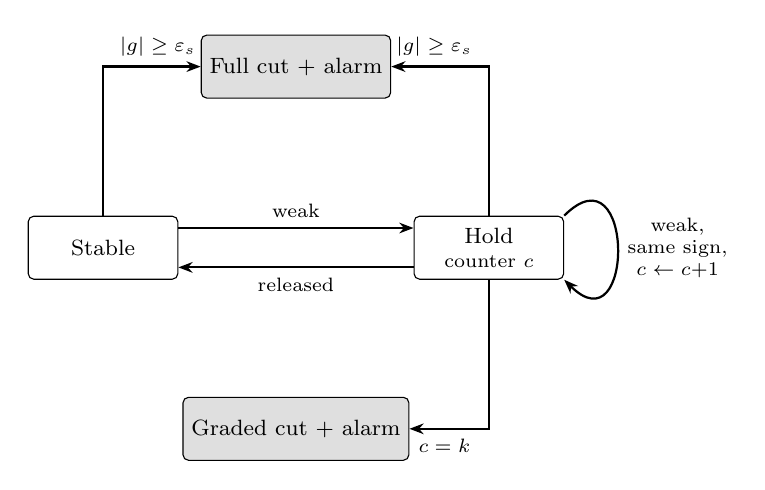
\begin{tikzpicture}[
  st/.style={draw, rounded corners=2pt, align=center, minimum height=8mm, minimum width=1.9cm, inner sep=3pt, font=\footnotesize, fill=white},
  ac/.style={draw, rounded corners=2pt, align=center, minimum height=8mm, inner sep=3pt, font=\footnotesize, fill=gray!25},
  arr/.style={-{Stealth[length=1.8mm]}, thick},
  lab/.style={font=\scriptsize, align=center}
]
\node[st] (stable) at (0,0) {Stable};
\node[st] (hold) at (4.9,0) {Hold\\[-1pt]{\scriptsize counter $c$}};
\node[ac] (full) at (2.45,2.3) {Full cut + alarm};
\node[ac] (grad) at (2.45,-2.3) {Graded cut + alarm};
\draw[arr] (stable.north) |- node[lab, pos=0.78, above] {$|g|\ge\varepsilon_s$} (full.west);
\draw[arr] (hold.north) |- node[lab, pos=0.78, above] {$|g|\ge\varepsilon_s$} (full.east);
\draw[arr] ([yshift=2.5mm]stable.east) -- node[lab, above] {weak} ([yshift=2.5mm]hold.west);
\draw[arr] ([yshift=-2.5mm]hold.west) -- node[lab, below] {released} ([yshift=-2.5mm]stable.east);
\draw[arr] (hold.south) |- node[lab, pos=0.78, below] {$c=k$} (grad.east);
\draw[arr] (hold.north east) .. controls +(0.9,0.9) and +(0.9,-0.9) .. node[lab, right, pos=0.5] {weak,\\same sign,\\$c\leftarrow c{+}1$} (hold.south east);
\end{tikzpicture}
% \caption{All states of the window-selection policy. A strong gap always triggers a full cut. A weak gap starts a hold which ends in a graded cut after $k$ consistent checks or is released when the gap vanishes or changes sign. After either cut the policy returns to Stable.}
  \caption{All states of the window-selection policy. A strong gap triggers an immediate full cut whereas a weak gap starts a hold period. A graded cut is applied after $k$ consecutive checks with consistent results while the hold is released if the gap disappears or changes sign.}
\label{fig:states}
\end{figure}

The graded cut removes only the oldest portion of $W_1$.  The removed share is $\rho=\min(1,|g|/\varepsilon_s)$ so larger gap removes a larger portion (Fig.~\ref{fig:cuts}). The expected benefit is that a gradual or small drift may keep $|g|$ below $\varepsilon_s$ for a long time even when the old data already differ from the new data. A weak gap that continues over time indicates this change and the hold state prevents a one-time unusual result from causing a cut.

\begin{figure}[!t]
\centering
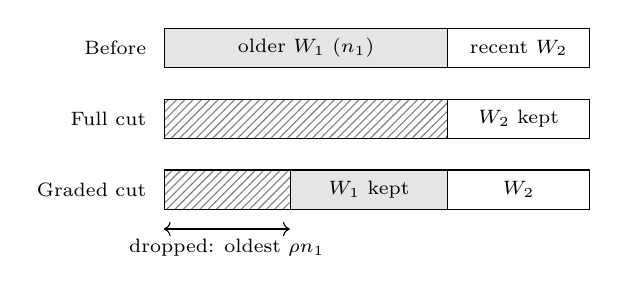
\begin{tikzpicture}[
  seg/.style={draw, minimum height=5mm, inner sep=0pt, font=\scriptsize},
  lab/.style={font=\scriptsize, anchor=east}
]
\def\a{3.6} \def\b{1.8} \def\d{1.6} \pgfmathsetmacro{\r}{\a-\d}
\node[lab] at (0,0) {Before};
\node[seg, minimum width=\a cm, fill=gray!20, anchor=west] (a1) at (0.1,0) {older $W_1$ ($n_1$)};
\node[seg, minimum width=\b cm, fill=white, anchor=west] (a2) at (\a+0.1,0) {recent $W_2$};
\node[lab] at (0,-0.9) {Full cut};
\node[seg, minimum width=\a cm, pattern=north east lines, pattern color=black!50, anchor=west] at (0.1,-0.9) {};
\node[seg, minimum width=\b cm, fill=white, anchor=west] at (\a+0.1,-0.9) {$W_2$ kept};
\node[lab] at (0,-1.8) {Graded cut};
\node[seg, minimum width=\d cm, pattern=north east lines, pattern color=black!50, anchor=west] at (0.1,-1.8) {};
\node[seg, minimum width=\r cm, fill=gray!20, anchor=west] at (\d+0.1,-1.8) {$W_1$ kept};
\node[seg, minimum width=\b cm, fill=white, anchor=west] at (\a+0.1,-1.8) {$W_2$};
\draw[<->, thin] (0.1,-2.3) -- node[font=\scriptsize, below] {dropped: oldest $\rho n_1$} (\d+0.1,-2.3);
\end{tikzpicture}
\caption{Window after a full cut (all of $W_1$ dropped, hatched) and after a graded cut (only the oldest part of $W_1$ dropped).}
\label{fig:cuts}
\end{figure}

If $\delta_w=\delta_s$ then the weak zone is empty and the policy equals ADWIN-U. So ADWIN-U is a special case. The policy adds only a counter and a sign per check and cuts whole buckets so we expect ADWIN-U's $O(\log W)$ cost to remain which we will measure. The lax test does not carry the strict bound's false-alarm guarantee once persistence is used so we will measure false alarms on drift-free streams. The parameters $\delta_s$, $\delta_w$, $k$, and $\rho$ are open choices to tune and ablate.

\subsection{Evaluation plan}

\paragraph{Datasets}
Table~\ref{tab:data} lists the datasets. We build drift on AG News \cite{zhang2015} by changing the topic mix. We use a single switch for abrupt drift, a sigmoid transition for gradual drift \cite{bifet2010} and a return to an earlier mix for recurring drift. On 20 Newsgroups \cite{lang1995}, swapping groups from different macro-topics gives strong drift and swapping sibling groups gives subtle drift. As a real stream we use timestamped Amazon reviews \cite{ni2019} in time order. Its drift points are unknown so we use proxies such as alarm rate downstream accuracy for a given label budget and alignment with a known event. Together the three datasets cover different types of text such as news, discussion posts and reviews. They also include different levels of label certainty from known injected drift points to unknown real drift points.

\begin{table}[!t]
\centering
\caption{Planned datasets.}
\label{tab:data}
\small
\begin{tabular}{>{\raggedright\arraybackslash}p{1.85cm}>{\raggedright\arraybackslash}p{3.6cm}>{\raggedright\arraybackslash}p{1.4cm}}
\toprule
Dataset & Role & Drift truth \\
\midrule
AG News & Abrupt, gradual, recurring drift by topic mix & Known \\
20 Newsgroups & Strong vs.\ subtle drift via macro-topics or sibling groups & Known \\
Amazon reviews & Real stream in time order & Unknown \\
\bottomrule
\end{tabular}
\end{table}

\paragraph{Baselines and metrics}
We compare against ADWIN-U (single and multiple detectors), plain ADWIN with a grid of $\delta$ values, a two-threshold warning/alarm variant, a KSWIN-style fixed-window test \cite{raab2020} and a D3-style discriminative detector \cite{gozuacik2019}. The $\delta$ grid and the warning/alarm variant test whether any gain comes only from tuning $\delta$ or adding a warning zone. We evaluate each detector using mean time to detection, false alarms per 1,000 instances, missed-drift rate, window length, per-instance latency and peak memory. We also report throughput in documents per second for showing that the detector keeps up with the stream. BAR \cite{assis2025} is used as an additional measure. First the detectors are set to the same false-alarm rate on a stream with no drift. Then they are tested on several random stream orders and ranked using the Friedman and Nemenyi tests \cite{demsar2006}. Ablation studies (hold only, graded cut without persistence and full policy) help to identify which part has the most impact.
%--------------------------------------------------------------------
%--------------------------------------------------------------------
\begin{thebibliography}{99}
\bibitem{gama2014} J.~Gama, I.~\v{Z}liobait\.{e}, A.~Bifet, M.~Pechenizkiy, and A.~Bouchachia, ``A survey on concept drift adaptation,'' \emph{ACM Comput.\ Surv.}, vol.~46, no.~4, art.~44, 2014, \doi{10.1145/2523813}.

\bibitem{lu2019} J.~Lu, A.~Liu, F.~Dong, F.~Gu, J.~Gama, and G.~Zhang, ``Learning under concept drift: A review,'' \emph{IEEE Trans.\ Knowl.\ Data Eng.}, vol.~31, no.~12, pp.~2346--2363, 2019, \doi{10.1109/TKDE.2018.2876857}.

\bibitem{garcia2024review} C.~M. Garcia, R.~Abilio, A.~L. Koerich, A.~S. Britto~Jr., and J.~P. Barddal, ``Concept drift adaptation in text stream mining settings: A systematic review,'' \emph{ACM Trans.\ Intell.\ Syst.\ Technol.}, vol.~16, no.~2, pp.~1--67, 2025, \doi{10.1145/3704922}.

\bibitem{hinder2024a} F.~Hinder, V.~Vaquet, and B.~Hammer, ``One or two things we know about concept drift---a survey on monitoring in evolving environments. Part A: Detecting concept drift,'' \emph{Front.\ Artif.\ Intell.}, vol.~7, art.~1330257, 2024, \doi{10.3389/frai.2024.1330257}.

\bibitem{lukats2025} D.~Lukats, O.~Zielinski, A.~Hahn, and F.~Stahl, ``A benchmark and survey of fully unsupervised concept drift detectors on real-world data streams,'' \emph{Int.\ J.\ Data Sci.\ Anal.}, vol.~19, pp.~1--31, 2025, \doi{10.1007/s41060-024-00620-y}.

\bibitem{bifet2007} A.~Bifet and R.~Gavald\`a, ``Learning from time-changing data with adaptive windowing,'' in \emph{Proc.\ SIAM Int.\ Conf.\ Data Mining}, 2007, pp.~443--448, \doi{10.1137/1.9781611972771.42}.

\bibitem{assis2025} D.~N. Assis and V.~M.~A. Souza, ``ADWIN-U: Adaptive windowing for unsupervised drift detection on data streams,'' \emph{Knowl.\ Inf.\ Syst.}, vol.~67, no.~11, pp.~10005--10034, 2025, \doi{10.1007/s10115-025-02523-1}.

\bibitem{webb2016} G.~I. Webb, R.~Hyde, H.~Cao, H.~L. Nguyen, and F.~Petitjean, ``Characterizing concept drift,'' \emph{Data Min.\ Knowl.\ Discov.}, vol.~30, no.~4, pp.~964--994, 2016, \doi{10.1007/s10618-015-0448-4}.

\bibitem{suarez2023} A.~L. Su\'arez-Cetrulo, D.~Quintana, and A.~Cervantes, ``A survey on machine learning for recurring concept drifting data streams,'' \emph{Expert Syst.\ Appl.}, vol.~213, art.~118934, 2023, \doi{10.1016/j.eswa.2022.118934}.

\bibitem{gama2004} J.~Gama, P.~Medas, G.~Castillo, and P.~Rodrigues, ``Learning with drift detection,'' in \emph{Advances in Artificial Intelligence (SBIA)}, LNAI vol.~3171, 2004, pp.~286--295, \doi{10.1007/978-3-540-28645-5_29}.

\bibitem{raab2020} C.~Raab, M.~Heusinger, and F.-M. Schleif, ``Reactive soft prototype computing for concept drift streams,'' \emph{Neurocomputing}, vol.~416, pp.~340--351, 2020, \doi{10.1016/j.neucom.2019.11.111}.

\bibitem{gozuacik2019} \"O.~G\"oz\"ua\c{c}\i k, A.~B\"uy\"uk\c{c}ak\i r, H.~Bonab, and F.~Can, ``Unsupervised concept drift detection with a discriminative classifier,'' in \emph{Proc.\ ACM Int.\ Conf.\ Inf.\ Knowl.\ Manag. (CIKM)}, 2019, pp.~2365--2368, \doi{10.1145/3357384.3358144}.

\bibitem{hoeffding1963} W.~Hoeffding, ``Probability inequalities for sums of bounded random variables,'' \emph{J.\ Amer.\ Statist.\ Assoc.}, vol.~58, no.~301, pp.~13--30, 1963, \doi{10.1080/01621459.1963.10500830}.

\bibitem{datar2002} M.~Datar, A.~Gionis, P.~Indyk, and R.~Motwani, ``Maintaining stream statistics over sliding windows,'' \emph{SIAM J.\ Comput.}, vol.~31, no.~6, pp.~1794--1813, 2002, \doi{10.1137/S0097539701398363}.

\bibitem{hinder2020} F.~Hinder, A.~Artelt, and B.~Hammer, ``Towards non-parametric drift detection via dynamic adapting window independence drift detection (DAWIDD),'' in \emph{Proc.\ Int.\ Conf.\ Mach.\ Learn.\ (ICML)}, PMLR vol.~119, 2020, pp.~4249--4259.

\bibitem{chen2024} J.~Chen, S.~Yang, T.~Gao, Y.~Ying, T.~Li, and P.~Li, ``Multi-type concept drift detection under a dual-layer variable sliding window in frequent pattern mining with cloud computing,'' \emph{J.\ Cloud Comput.}, vol.~13, art.~40, 2024, \doi{10.1186/s13677-023-00566-9}.

\bibitem{klinkenberg2000} R.~Klinkenberg and T.~Joachims, ``Detecting concept drift with support vector machines,'' in \emph{Proc.\ Int.\ Conf.\ Mach.\ Learn.\ (ICML)}, 2000, pp.~487--494.

\bibitem{kuncheva2009} L.~I. Kuncheva and I.~\v{Z}liobait\.{e}, ``On the window size for classification in changing environments,'' \emph{Intell.\ Data Anal.}, vol.~13, no.~6, pp.~861--872, 2009, \doi{10.3233/IDA-2009-0397}.

\bibitem{mehmood2024} H.~Mehmood, A.~Khalid, P.~Kostakos, E.~Gilman, and S.~Pirttikangas, ``A novel edge architecture and solution for detecting concept drift in smart environments,'' \emph{Future Gener.\ Comput.\ Syst.}, vol.~150, pp.~127--143, 2024, \doi{10.1016/j.future.2023.08.023}.

\bibitem{badar2023} M.~Badar, W.~Nejdl, and M.~Fisichella, ``FAC-fed: Federated adaptation for fairness and concept drift aware stream classification,'' \emph{Mach.\ Learn.}, vol.~112, pp.~2761--2786, 2023, \doi{10.1007/s10994-023-06360-7}.

\bibitem{hu2024} L.~Hu, W.~Li, Y.~Lu, and C.~Hu, ``Scalable concept drift adaptation for stream data mining,'' \emph{Complex Intell.\ Syst.}, vol.~10, pp.~6725--6743, 2024, \doi{10.1007/s40747-024-01524-x}.

\bibitem{reimers2019} N.~Reimers and I.~Gurevych, ``Sentence-BERT: Sentence embeddings using Siamese BERT-networks,'' in \emph{Proc.\ EMNLP-IJCNLP}, 2019, pp.~3980--3990, \doi{10.18653/v1/D19-1410}.

\bibitem{wang2020} W.~Wang, F.~Wei, L.~Dong, H.~Bao, N.~Yang, and M.~Zhou, ``MiniLM: Deep self-attention distillation for task-agnostic compression of pre-trained transformers,'' in \emph{Advances in Neural Information Processing Systems}, vol.~33, 2020.

\bibitem{zhang2015} X.~Zhang, J.~Zhao, and Y.~LeCun, ``Character-level convolutional networks for text classification,'' in \emph{Advances in Neural Information Processing Systems}, vol.~28, 2015.

\bibitem{lang1995} K.~Lang, ``NewsWeeder: Learning to filter netnews,'' in \emph{Proc.\ Int.\ Conf.\ Mach.\ Learn.\ (ICML)}, 1995, pp.~331--339, \doi{10.1016/B978-1-55860-377-6.50048-7}.

\bibitem{ni2019} J.~Ni, J.~Li, and J.~McAuley, ``Justifying recommendations using distantly-labeled reviews and fine-grained aspects,'' in \emph{Proc.\ EMNLP-IJCNLP}, 2019, pp.~188--197, \doi{10.18653/v1/D19-1018}.

\bibitem{bifet2010} A.~Bifet, G.~Holmes, R.~Kirkby, and B.~Pfahringer, ``MOA: Massive online analysis,'' \emph{J.\ Mach.\ Learn.\ Res.}, vol.~11, pp.~1601--1604, 2010.

\bibitem{demsar2006} J.~Dem\v{s}ar, ``Statistical comparisons of classifiers over multiple data sets,'' \emph{J.\ Mach.\ Learn.\ Res.}, vol.~7, pp.~1--30, 2006.
\end{thebibliography}

\end{document}
